\section{Results of Part 2}

\subsection{Question A}
The bubble sort function was created based off of sudo code for a generalised bubble sort.
The code is shown below

\begin{Matlab}
 function array = BubbleSort(array)
  for i = 1:length(array)
   for j = length(array):-1:i+1
    if array(j) > array(j-1)
     temp = array(j);
     array(j) = array(j-1);
     array(j-1) = temp;
    end
   end
  end
 return;
 end
\end{Matlab}

This code took 0.0087 seconds to sort the 100x100 matrix

\subsection{Question B}
The code to test the user function is shown below.
'timetaken' is a matrix for storing the times of both the user and inbuilt functions.

\begin{Matlab}
 % Initialize the cell array
 testsizes = [100; 200; 500; 1000; 1200];
 timetaken = cell(1+length(testsizes),4);
 timetaken(1,:) = {"size", "bubble sort time", "inbuilt sort time", "speed up"};
 timetaken(2:end,1) = num2cell(testsizes); % should use [100; 200; 500; 1000; 10000] but takes too long so using 1100 for know

 % Loop over each row in timetaken
 for i = 2:size(timetaken,1)
  % Call the timetest function with the value in the first column of the i-th row
  [timeBubble, timeInbuilt] = timetest(timetaken{i,1});
  timetaken{i,2} = timeBubble;
  timetaken{i,3} = timeInbuilt;
  % Calculate speed up
  timetaken{i,4} = timeBubble/timeInbuilt;
 end
 % Display the results
 disp(timetaken)
\end{Matlab}

The function 'timetest' is given below.
It takes a matrix size, creates a square matrix, and then outputs the sort time for both the user and inbuilt functions.

\begin{Matlab}
 function [t_user,t_inbulit ] = timetest(size)

  X=rand(size, size);
  Y=X;

  tic
  for i = 1:size
   X(:,i) = BubbleSort(X(:,i));
  end
  t_user = toc();

  tic
  for i = 1:size
   Y(:,i) = sort(Y(:,i));
  end
  t_inbulit = toc();

  display("Time tacken by the bubble sort function was " + t_user + " s. Time tacken by the inbuilt sort function was: "+  t_inbulit +" s.")

  return;
 end
\end{Matlab}

The results from the tests are shown in the table below

\Table{User vs inbuilt sort function}{lrrr}{
 \textbf{Matrix size} & \textbf{User} & \textbf{Inbuilt} & \textbf{Speed up}
}{
 100 & 0.0087 & 0.0002 & 40.507 \\
 200 & 0.0205 & 0.0003 & 62.791 \\
 500 & 0.1780 & 0.0012 & 145.18 \\
 1000 & 2.1324 & 0.0048 & 445.16 \\
 1000 & 1813.9 & 1.5631 & 1160.4 \\
}{2btbl}

\begin{figure}[H]
 \centering
 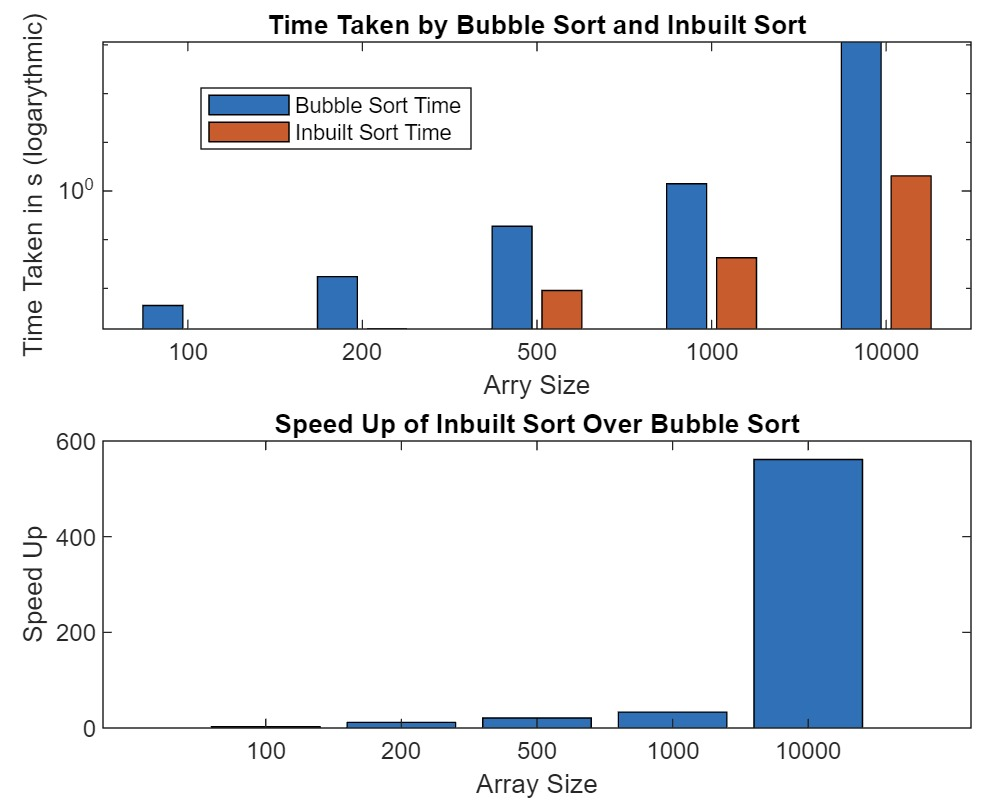
\includegraphics[width=0.6\columnwidth]{Figures/noPar}
 \caption{User vs inbuilt sort function}
 \label{fig:noPar}
\end{figure}

WHYYYYY

\subsection{Question C}
The code to test the parallelism  user function is shown below.
'timetaken' is a matrix for storing the times of both the user and inbuilt functions.

\begin{Matlab}% Initialize the cell array
 testsizes = [100, 5000];
 timetaken_par = cell(1+length(testsizes),4);
 timetaken_par(1,:) = {"size", "bubble sort time", "inbuilt sort time", "speed up"};
 timetaken_par(2:end,1) = num2cell(testsizes); % should use [100; 200; 500; 1000; 10000] but takes too long so using 1100 for know

 % Loop over each row in timetaken_par
 for i = 2:size(timetaken_par,1)
  % Call the timetest function with the value in the first column of the i-th row
  timeBubble = timebubble_parallelism(timetaken_par{i,1});
  timeInbuilt = timesort_parallelism(timetaken_par{i,1});
  timetaken_par{i,2} = timeBubble;
  timetaken_par{i,3} = timeInbuilt;
  % Calculate speed up
  timetaken_par{i,4} = timeBubble/timeInbuilt;
 end

 % Display the results
 disp(timetaken_par)
\end{Matlab}

The function 'timesort\_parallelism' simply returns the time to sort a square matrix of a given size using the inbuilt sort function.
The function 'timebubble\_parallelism' is given below.
It takes a matrix size, creates a square matrix, and then outputs the sort time for the user parallelism bubble-sort function.

\begin{Matlab}
 function t_user = timebubble_parallelism(size)

  X=rand(size, size);

  tic
  spmd
   myStart = (spmdIndex - 1) * 25 + 1;
   myEnd = myStart + 24;
   for i = myStart:myEnd
    X(:,i) = BubbleSort(X(:,i));
   end
  end
  t_user = toc();

  display("Time tacken by the parallelism bubble sort function was " + t_user )

  return;
 end
\end{Matlab}

The results from the tests are shown in the table below

\Table{User vs inbuilt sort function}{lrrr}{
 \textbf{Matrix size} & \textbf{User} & \textbf{Inbuilt} & \textbf{Speed up}
}{
 100 & 0.7921 & 0.0011 & 690.97 \\
 5000 & 0.2.1446 & 0.4808 & 4.4607 \\
}{2ctbl}

\begin{figure}[H]
 \centering
 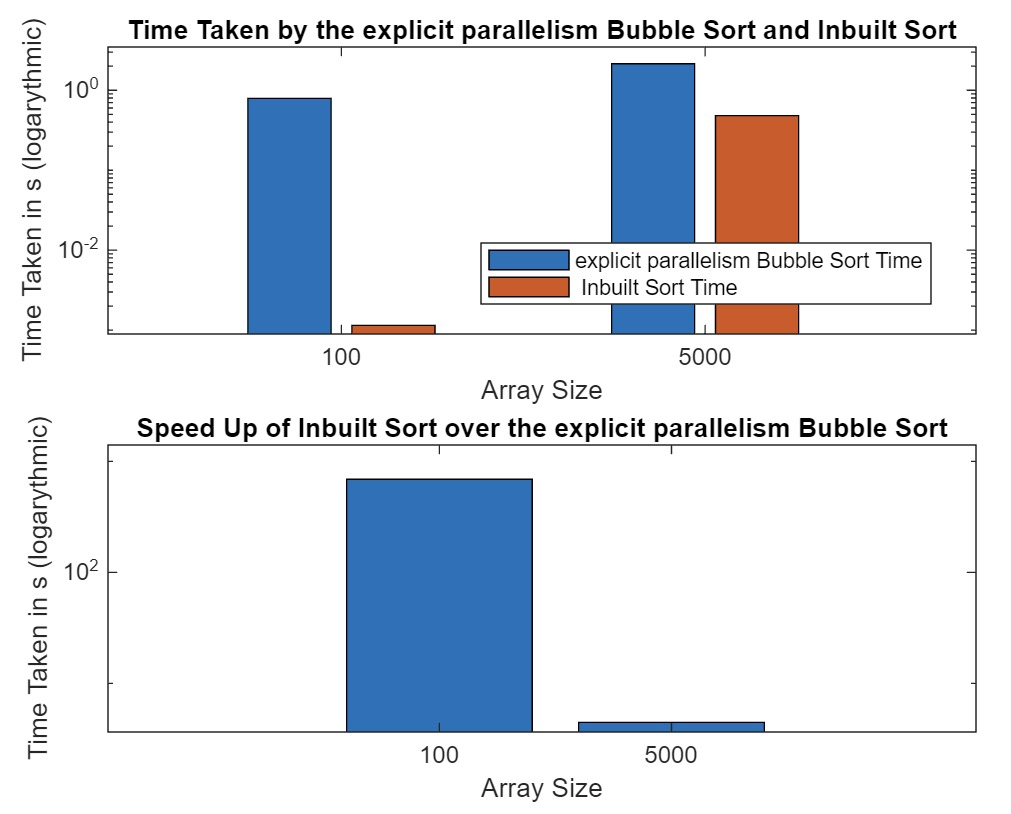
\includegraphics[width=0.6\columnwidth]{Figures/expPar}
 \caption{User parallelism vs inbuilt sort function}
 \label{fig:expPar}
\end{figure}

WHYYYY